\section{Der Speicher}
\index{Speichermodell}
\label{sec:Speicher}

Beim Hochfahren der Maschine wir der komplette Speicher mit dem
Wert Null initialisiert und anschließend das angegebene Maschinenprogramm in den
Speicher geladen. Die Größe des Speichers ist nicht festgelegt.



\subsection{Speicherstruktur}
\label{subsec:Speicherstruktur}
\index{Speicherstruktur}

Der Speicher der UMach Maschine hat zur Laufzeit eine bestimmte Struktur, bzw.
wird in bestimmten Bereichen unterteilt. Diese Bereiche sind
\begin{enumerate}
 \item Interrupttabelle
 \item Programm und Daten
 \item Stack
\end{enumerate}

Siehe auch die Abbildung \ref{fig:Speicherstruktur} auf der Seite
\pageref{fig:Speicherstruktur}.

\begin{figure}[htp]
 \centering
 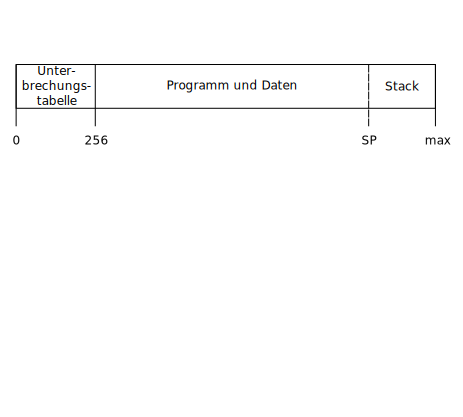
\includegraphics{./img/UMach-Speicherstruktur}
 \caption[Speicherstruktur]{Speicherstruktur zur Laufzeit}
 \label{fig:Speicherstruktur}
\end{figure}



\subsubsection{Interrupttabelle}
\index{Interrupttabelle}
\label{subsubsec:Interrupttabelle}

Die Interrupttabelle besteht aus einer Reihe von 32-Bit langen Sprungadressen
zum ausführbaren Code, bzw. zu sogenannten Interruptroutinen, oder auch \glqq
Interrupt Handlers\grqq, die in Ausnahmefällen ausgeführt werden sollen. Jedes
mal, wenn eine Ausnahmesituation auftritt (meistens eine Fehlersituation), wird
intern ein Interruptsignal erzeugt, das mit einer Kennnummer (Interruptnummer)
versehen ist. Die Interruptnummer wird als Index in dieser Tabelle verwendet.


Die Interrupttabelle wird nicht von der Maschine nicht gefüllt, sondern es ist
Aufgabe des Maschinenprogramms bei bedarf entsprechende Einträge der
Interrupttabelle zu füllen und die zugehörige Funktionalität bereit zu stellen.
Ist eine Interrupadresse nicht gesetzt, d.h. ist der entsprechende
Tabelleneintrag Null, so reagiert die Maschine auf die Ausnahmesituation
in dem sie hält. Für weitere Informationen bzgl. der Fehlerbehandlung siehe den
Abschnitt \ref{sec:Interrupts}, ab der Seite \pageref{sec:Interrupts}.

Die Interrupttabelle besteht aus 64 Einträgen, was 64 möglichen Interrupts
entspricht. Jeder Eintrag beträgt wie ein Register 32 Bit, oder 4 Byte. Da es
64 Einträge gibt, ist die Interrupttabelle $64 \cdot 4 = 256$ Bytes groß. Die
Interrupttabelle fängt an der Adresse Null an. Siehe auch Abbildung
\ref{fig:Speicherstruktur} auf Seite \pageref{fig:Speicherstruktur}.


Tabelle \ref{tab:Interrupttabelle} auf Seite
\pageref{tab:Interrupttabelle} listet alle definierten
Interruptnummer\index{Interruptnummer} und deren Bedeutung auf.


\subsubsection{Programm und Daten}
\index{Programm}

Nach der $256$ Bytes ($64$ mal $4$) großen Interrupttabelle
folgt das eigentliche Programm, das von der Maschine ausgeführt werden soll.
Dieses erste auzuführende Programm beginnt somit ab der Speicheradresse $256$.

Insbesondere ist dieses Programm dafür zuständig, die Interrupttabelle zu
füllen, falls (bestimmte) Interrupts behandelt werden sollen.



\subsubsection{Der Stack}
\label{subsubsec:Stack}
\index{Stack}

Der Stack ist ein spezieller Bereich im Speicher. Dieser Bereich fängt am Ende
des Speichers mit der größten Adresse an und erstreckt sich bis zur derjenigen
Adresse, die im Register \texttt{SP} gespeichert ist. Die Stack-Größe ist damit
dynamisch, denn das Register \texttt{SP} wird sowohl durch die Instruktionen
\opref{PUSH} und \opref{POP}, als auch direkt vom Programmierer geändert.

Das Wachsen\index{Stack!Wachsen} des Stacks bedeutet, dass das Register
\texttt{SP} immer kleinere Werte annimmt. Das Schrumpfen\index{Stack!Schrumpfen}
des Stacks bedeutet, dass \texttt{SP} immer größere Werte annimmt. Wird
versucht, den Inhalt von \texttt{SP} kleiner Null oder größer als die maximale
Speicheradresse zu setzen, so wird dies von der Maschine verweigert und als
Fehler im Register \texttt{ERR} signalisiert.

Beim Hochfahren der Maschine, wird das Register \texttt{SP} auf die
maximal erreichbare Speicheradresse plus Eins gesetzt. Damit können keine Werte
gelesen werden, bevor Werte geschrieben wurden.


\subsection{Speicheradressierung}
\index{Speicheradresse}

Um die Komplexität der UMach Maschine gering zu halten, kennt die vorliegende
Version lediglich absolute Adressen. Konzepte wie virtuelle Adressen,
Prozesse\index{Prozess} und getrennte Addressräume für Prozesse werden nicht
unterstützt. Wird versucht, den Inhalt einer Speicheradresse zu lesen oder zu
schreiben, so wird die angegebene Adresse nicht übersetzt oder modifiziert,
sondern direkt verwendet.

